\appendix
\section{Ergaenzende Abbildungen}

\begin{figure}[H]
\centering
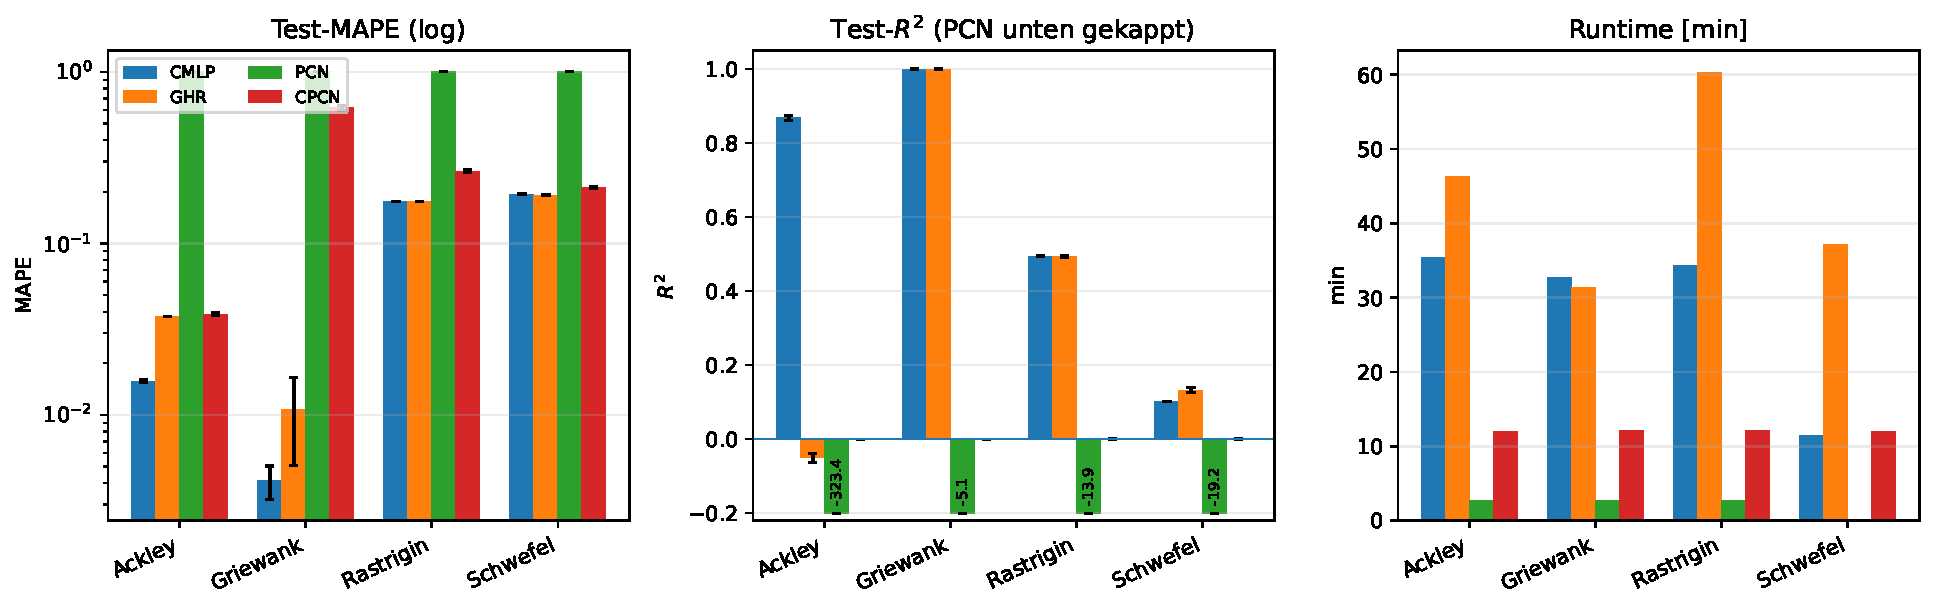
\includegraphics[width=0.95\textwidth]{graphics/generated/holdout_comparison.pdf}
\caption{Vergleich der Holdout-Metriken für CMLP, GHR, PCN und CPCN. CMLP und GHR verwenden fünf Wiederholungen, CPCN zehn Wiederholungen und PCN eine Wiederholung pro Funktion.}
\label{fig:holdout-comparison}
\end{figure}

\begin{figure}[H]
\centering
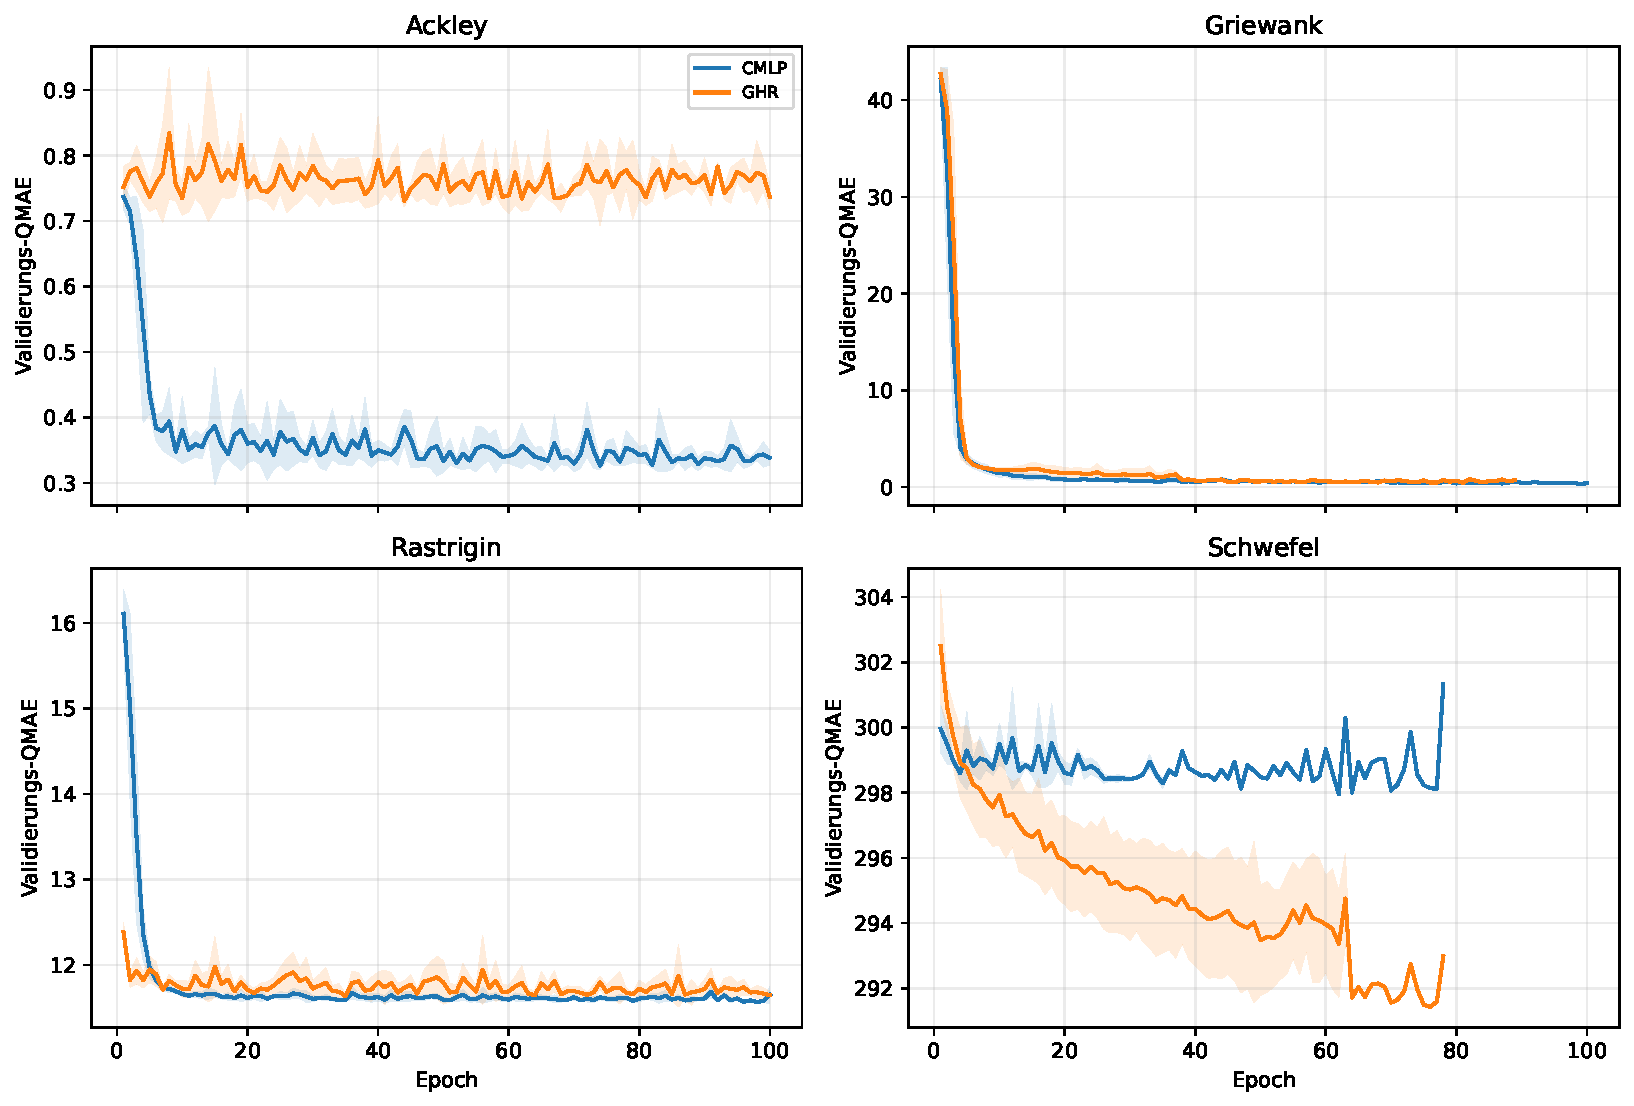
\includegraphics[width=0.95\textwidth]{graphics/generated/learning_curves_cmlp_ghr.pdf}
\caption{Validierungs-QMAE der Quaternion-Baselines. CMLP zeigt auf mehreren Funktionen eine schnelle Anfangsverbesserung und danach langsamere weitere Verbesserung.}
\label{fig:learning-curves}
\end{figure}

\begin{figure}[H]
\centering
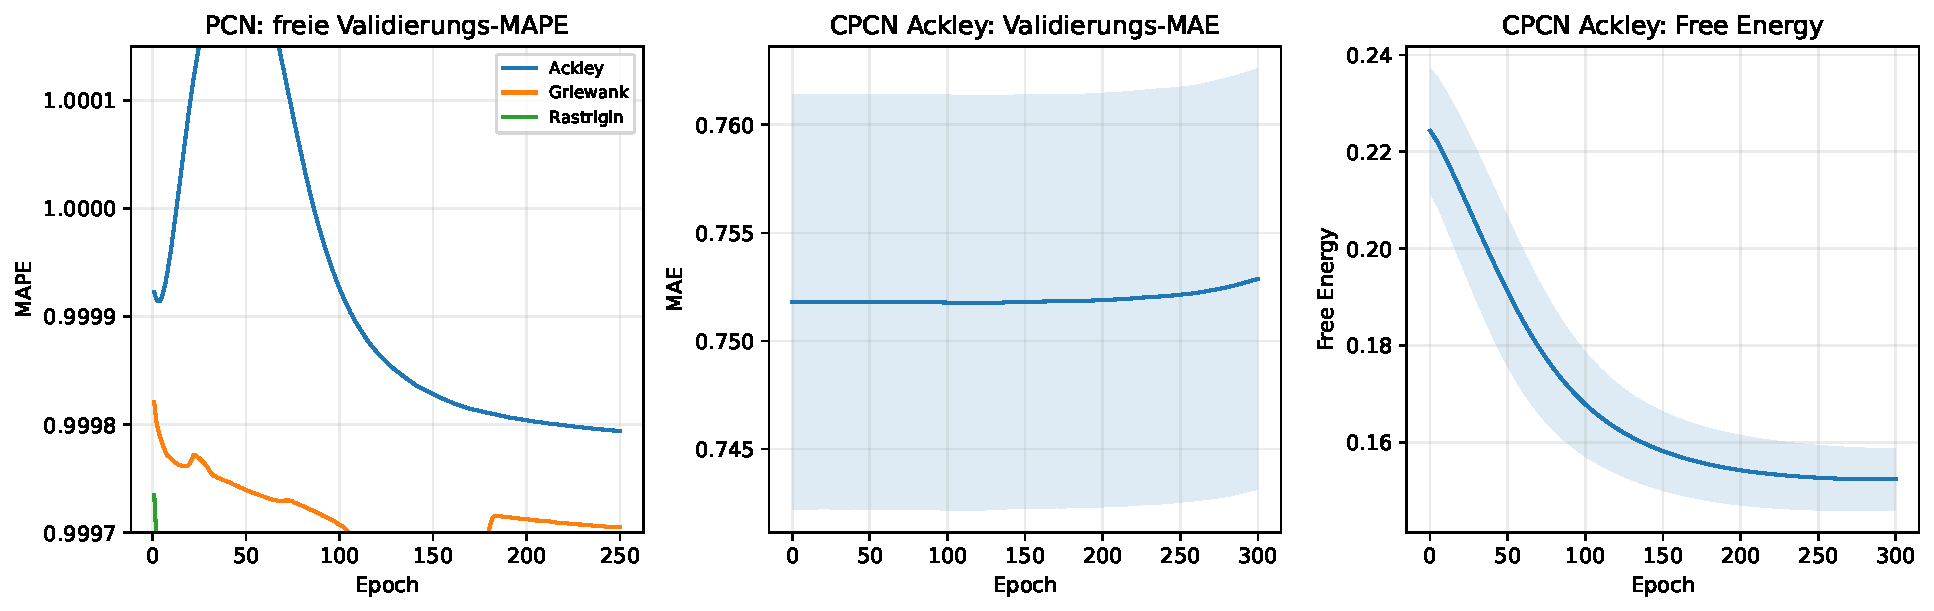
\includegraphics[width=0.95\textwidth]{graphics/generated/pcn_cpcn_training_behavior.pdf}
\caption{Optimierungsverhalten der PC-basierten Modelle am Beispiel Ackley. Beim reellwertigen PCN bleibt die freie Validierungs-MAPE nahe 1.0. Beim CPCN sinkt die Free Energy sichtbar, während die Validierungs-MAE nur sehr langsam reagiert.}
\label{fig:pcn-cpcn}
\end{figure}

\section{Hinweise zu Code und Artefakten}

Die wichtigsten Artefakte liegen in folgenden Ordnern:
\begin{itemize}
    \item \texttt{src/qvnn\_pc/}: Implementierung der Benchmark-Funktionen, Datensplits, Quaternion-Operationen, CMLP, GHR, PCN und CPCN.
    \item \texttt{notebooks/}: Sanity-Checks, Reproduktion der Baselines, PCN-Diagnostik, MNIST-Probe und Auswertung gespeicherter Resultate.
    \item \texttt{results/}: gespeicherte CSV-Zusammenfassungen, Lernverlaeufe, Modelle und generierte Plots.
    \item \texttt{cluster/}: SLURM-Skripte für laengere Benchmark-Laeufe.
\end{itemize}

Der Bericht verwendet für die Tabellen im Hauptteil die finalen Resultate aus \texttt{results/archcmp\_resume/}, \texttt{results/pcn-h200/} und \texttt{results/cpcn-h200/}. Der Schwefel-Lauf des reellwertigen PCN ist als \texttt{non\_finite} markiert und wird deshalb nicht als erfolgreiches Training interpretiert.
